%%%%%%%%%%%%%%%%%%%%%%%%%%%%%%%%%%%%%%%%	
\subsection{RVSI: Snapshot Isolation 一致性弱化与维护}

\newcommand{\chameleon}{\textsc{Chameleon}}
%%%%%%%%%%%%%%%
\begin{frame}{RVSI 工作在技术框架中的位置}
  \fig{width = 0.50\textwidth}{figures/3d-framework-rvsi.pdf}
	{RVSI --- Snapshot Isolation 一致性弱化与维护.}
\end{frame}
%%%%%%%%%%%%%%%
\begin{frame}{研究动机}
  \question{问题: 为什么要提出 Relaxed Version Snapshot Isolation {\small (RVSI)} 一致性?}
  \vspace{0.20cm}

  \begin{description}
    \setlength{\itemsep}{5pt}
    \item[分布式事务:] 
      \begin{itemize}
        \item ``all-or-none'' 语义
        \item 受到分布式存储系统的关注 \citeinbeamer{Cassandra}{CASSANDRA-ISSUE-7056}{14}
      \end{itemize}
    \item[弱一致性:] 
      \begin{itemize}
        \item PCSI \citeinbeamer{Elnikety}{SRDS}{05} 
		  \textcolor{red}{SI} \citeinbeamer{Lin}{TODS}{09} \\
          PSI \citeinbeamer{Sovran}{SOSP}{11} NMSI \citeinbeamer{Ardekani}{SRDS}{13} 
        \end{itemize}
    \pause
	\item[\textcolor{red}{异常控制:}]
      \begin{itemize}
        \item 容忍``有限度的''异常 \citeinbeamer{Yu}{TOCS}{02}
      \end{itemize}
	\item[\textcolor{red}{可定制:}] 
      \begin{itemize}
        \item 不同应用对一致性需求不同 \citeinbeamer{Terry}{CACM}{13}
        \item 运行时决定 \citeinbeamer{Terry}{SOSP\&TR}{13}
      \end{itemize}
  \end{description}
 
  % \pause
  % \vspace{0.30cm}
  % \textcolor{black}{RVSI (Relaxed Version Snapshot Isolation):}
  % \begin{enumerate}
  %   \item 支持可定制一致性 
  %   \item 提供``有限度的''异常控制 
  % \end{enumerate}
\end{frame}
%%%%%%%%%%%%%%%
\begin{frame}{RVSI 定义}
  RVSI 定义原则:
  \begin{itemize}
    \item 参数 $k_1, k_2, k_3$ 控制``异常''程度
    \item $\text{RC} \supset \text{RVSI}(k_1, k_2, k_3) \supset \text{SI}$
    \item $\text{RVSI}(\infty,\infty,\infty) = \text{RC}; \qquad \text{RVSI}(1,0,\ast) = \text{SI}$
  \end{itemize}

  \vspace{0.20cm}

  \begin{cdef}[RVSI: Relaxed Version Snapshot Isolation]
    \begin{description}
      \item[单变量读 $\texttt{read}(x)$:] \hfill 
        \begin{enumerate}
          \item 允许读 $\le k_1$ 陈旧值
          \item 允许读 $\le k_2$ 并发更新
        \end{enumerate}
      \item[多变量读 $\texttt{read}(x), \texttt{read}{(y)}$:] \hfill
        \begin{enumerate}
          \setcounter{enumi}{2}
		\item $\text{distance}(\textsl{snap}{(x)},\textsl{snap}{(y)}) \le k_3$
        \end{enumerate}
    \end{description}
  \end{cdef}
\end{frame}
%%%%%%%%%%%%%%%
\begin{frame}{\chameleon{} 系统设计}
  \centerline{\textcolor{blue}{\chameleon{}: 
	支持数据分区与数据副本的分布式事务键值存储原型系统.}}

  \fig{width = 0.60\textwidth}{figures/chameleon-arch.pdf}{\chameleon 系统架构图.}
\end{frame}
%%%%%%%%%%%%%%%
\begin{frame}{\chameleon{} 系统设计}
  \centerline{\textcolor{blue}{\chameleon{}: 
	支持数据分区与数据副本的分布式事务键值存储原型系统.}}

  \fig{width = 0.45\textwidth}{figures/chameleon-framework.pdf}{\chameleon 系统组件图.}
\end{frame}
%%%%%%%%%%%%%%%
\begin{frame}{RVSI 维护算法}
  \[
    \textcolor{blue}{\text{RC} \supset \text{RVSI}(k_1, k_2, k_3) \supset \text{SI}}
  \]

  \vspace{0.10cm}

  RVSI 维护算法:
  \begin{itemize}
    \item 以分布式 RC 和 SI 协议 为基础
    \item 事务执行时, 添加 RVSI ``版本约束'' ($k_1, k_2, k_3$ 相关不等式)
    \item 事务提交时, 检查 RVSI ``版本约束''
  \end{itemize}

  % \fignocaption{width = 0.50\textwidth}{figures/chameleon-build-passing.png}
  \textcolor{red}{\small \url{https://github.com/hengxin/chameleon-transactional-kvstore}}
\end{frame}
%%%%%%%%%%%%%%%
\begin{frame}{RVSI 实验评估}
  \begin{figure}
	\begin{subfigure}{0.60\textwidth}
	  \centering
	  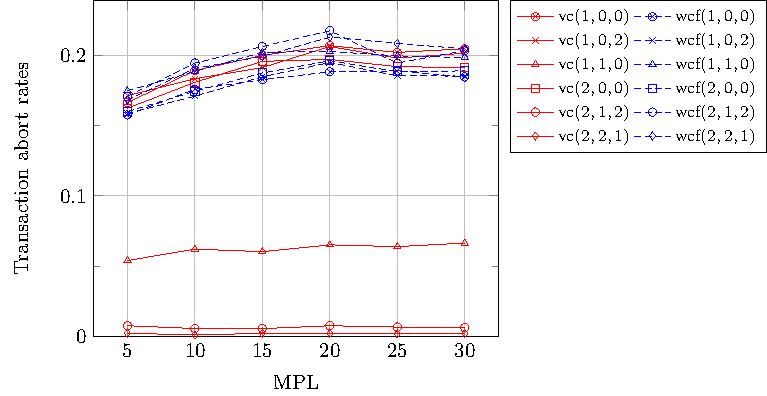
\includegraphics[width = 0.80\textwidth]{figures/rvsi-rw4-abort-rates.pdf}
	  \caption{rwRatio = 4:1.}
	\end{subfigure}%

	\begin{subfigure}{0.50\textwidth}
	  \centering
	  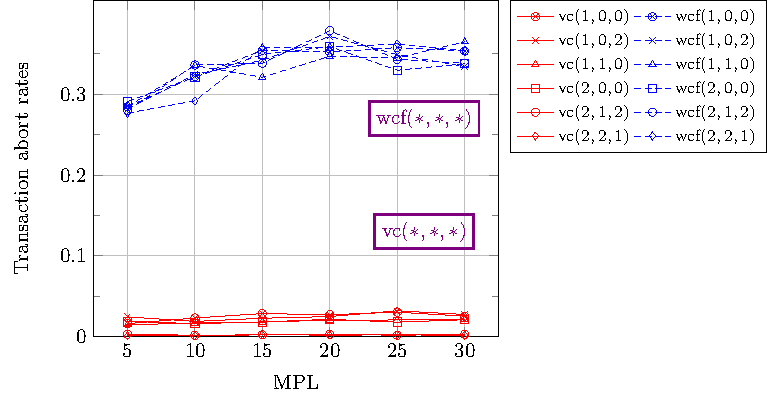
\includegraphics[width = 0.60\textwidth]{figures/rvsi-rw05-abort-rates.pdf}
	  \caption{rwRatio = 1:2.}
	\end{subfigure}%
	\begin{subfigure}{0.50\textwidth}
	  \centering
	  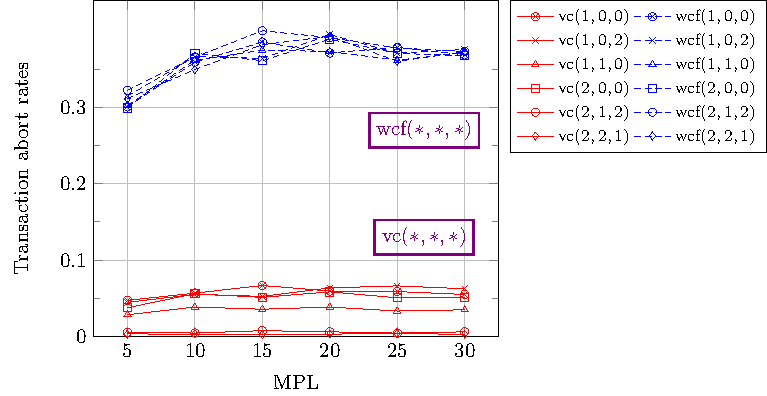
\includegraphics[width = 0.60\textwidth]{figures/rvsi-rw1-abort-rates.pdf}
	  \caption{rwRatio = 1:1.}
	\end{subfigure}%
	\caption{.}
  \end{figure}
\end{frame}
%%%%%%%%%%%%%%%
\begin{frame}{RVSI 的意义}
  \mdf{red}{blue}{}{teal}{
	\begin{itemize}
	  \item 运行时可调节
	  \item 适当放松事务对 RVSI 版本规约的要求可降低事务中止率
	  \item RVSI 能否``显著''降低事务中止率与负载类型相关
    \end{itemize}
  }
\end{frame}
%%%%%%%%%%%%%%%
